\begin{comment}
\subsection{Distributed-prover Zero-knowledge Protocols}
This discussion will formally define a zero-knowledge protocol which supports multiple proves and distributed proof generation.
\subsubsection{Definition of DPZK}
Consider a language $L \in \npol$ and the corresponding relation $R \in \pol$  \commentA{what is $\pol$} such that
\[
\stmt \in L \Leftrightarrow R(\stmt, \wit)=1 \text{ for some witness } \wit
\]
Let $\prover_1, \ldots, \prover_{\Num}$ be $\Num$ provers. In our setting, we let each party have an additive share of the witness $\wit$. For prover $i \in [\Num]$, let $\wit_i$ be its share.  The witness $\wit$ and its shares have length equal to the number of input wires of the circuit $\C$ representing the relation $R$. We will discuss later in this section why we decided to do an additive share of the witness. \commentA{the following didn't make sense to me}For now, note that a partition of the witness among the provers such that each prover owns a non-intersecting piece of the witness is a sub-class of additive sharing since the share of a prover can be its partition of the witness padded with zeros in the rest of positions.


A DPZK protocol consists of three probabilistic polynomial time algorithms: $(\setup, \Pi, \verifier)$. 
\begin{itemize}
\item $\setup$ takes as input the security parameter $1^\secp$ and optionally a trapdoor $\tau$ and outputs the public parameters $\sigma$ of the system.
\item The interactive proof system is an $\round$-round protocol $\langle \Pi = \{\pi_i\}_{i \in [\round]}, \verifier \rangle$ where in every round $i \in [\round]$, we have the output $m_i$ of $\pi_i(\st^i_1, \ldots, \st^i_{\Num})$ provided to $\verifier$. Here, $\st^i_j$ is the state of the prover $\prover_j$ at round $i$. $\st^1_j$ is set to $\prover_j$'s share of the witness $\wit_j$, randomness $r_j$, the public parameters $\sigma$ and updated later as the protocol proceeds. The output of $\verifier$ is either an $\tt accept$ (1) or a $\tt{reject}$ (0). Also, let $\tr$ be the transcript of the protocol.
\end{itemize}
A $\DPZK$ protocol for a language $L$ satisfies the following properties: 
correctness, soundness, zero-knowledge and privacy among provers.


\begin{comment}
\begin{myboxfig}{Ideal Functionality for Distributed ZK}{funcsabort}
	\begin{center}
		\textbf{ $\FDPZK$}
	\end{center}
	%Each honest party $P_i$ sends its input $x_i$ to the functionality. Corrupted parties may send the trusted party arbitrary inputs as instructed by the adversary. When sending the inputs to the trusted party, the adversary is allowed to send a special $\abort$ command as well.
	\begin{description}
	\item[--] $ $
	%	\item[\textbf{Input:}] On message $(\sid,\In, x_i$) from a party $P_i$ $(i \in [3])$, do the following: if $(\sid,\In, *)$ message was received from $P_i$, then ignore. Otherwise record $x_i' = x_i$ internally. 	If $x_i'$ is outside of the domain for $P_i$ $(i \in [3])$, consider $x_i' = \abort$. 
		
	%	\item[\textbf{Output to adversary:}] If there exists $i \in [3]$ such that $x_i' = \abort$, send $( \sid,\Output, \bot)$ to all the parties. Else, send $(\sid,\Output, y)$ to the adversary, where $y = f(x_1', x_2', x_3')$.
		
	%	\item[\textbf{Output to selected honest parties:}] 	Receive $(\select, \{I\})$ from adversary, where $\{I\}$ denotes a subset of the honest parties. %(where $\{I\}$ may denote empty set or ). If an honest party belongs to $I$, send $(\sid,\Output, y)$, else send $(\sid,\Output, \bot)$. 
		
		%		If there exists $i \in [3]$ such that $x_i' = \abort$, send $( \sid,\Output, \bot)$ to all the parties. Else, send $(\sid,\Output, y)$ to the corrupt party $P^*$, where $y = f(x_1', x_2', x_3')$.
		
	\end{description}
\end{myboxfig}

\commentA{I discussed with protik yesterday, it's better to change this to rael/ideal world setting.}
\dnote{self: give a name for Privacy among provers}
\paragraph{Completeness}: %We will define correctness assuming that the witness set is minimal.
Given $\sigma \gets \Setup(1^\secp, \tau)$ and a valid witness $\wit$ corresponding to $\stmt \in L$, when the initial states are set with $\sigma$ and the shares of $\wit$, $\langle \Pi, \verifier \rangle$ outputs 1 with probability 1.

\paragraph{Soundness}:  The basic definition of soundness ensures the existence of a valid witness for $\stmt \in L$. For every instance $\stmt \notin L$ and any $\ppt$ algorithm $\Pi^*$, $\verifier$ accepts with probability at most $\negl(\secp)$.

The notion of proof of knowledge of the witness by the prover is captured by the notion of knowledge extraction where an extractor extracts the witness whenever the verifier accepts using an oracle access to the prover. The stronger notion of witness extended emulation \cite{Lindell03} proposes the existence of an emulator which additionally produces a simulated transcript between the prover and the verifier irrespective of whether the verifier accepts or not. We will now define the notion of witness-extended emulation for the $\DPZK$ setting, adapted from \cite{Groth11}. 
%\commentA{I do not understand the below definition; two probabilities are indistinguishable? why is $\adv$ outputting one goven $\tr$???? same with remaining definitions}
\begin{definition}
The argument $(\Setup, \Pi, \verifier)$ has computational witness-extended emulation if for all deterministic polynomial time $\Pi^*$ there exists an expected polynomial time emulator $\chi$ such that for all non-uniform polynomial time adversaries $\adv$ and all $\tau$
\begin{align*}
& \pr \left[\sigma \leftarrow \Setup(1^\secp, \tau); (\stmt, \{\wit_i\}_{i \in [\Num]}) \leftarrow \adv(\sigma); \tr \leftarrow \langle \Pi^*, \verifier \rangle: \adv(\tr) = 1 \right] \\
\approx \; & \pr \left[\sigma \leftarrow \Setup(1^\secp, \tau); (\stmt, \{\wit_i\}_{i \in [\Num]}) \leftarrow \adv(\sigma); (\tr, \wit) \leftarrow \chi^{\langle \Pi^*, \verifier \rangle}(\sigma, x): \right. \\
&\;\;\; \adv(\tr) = 1 \left. \text{ and if } \tr \text{ accepts then } \stmt \in L \text{ with } \wit \text{ as witness} \right] 
\end{align*}

where $\chi$ has access to the oracle $\langle \Pi^*, \verifier \rangle$ which produces the transcript. $\chi$ can rewind $\langle \Pi^*, \verifier \rangle$ to any round and resume the protocol with fresh randomness from the verifier.
\end{definition}
%.\dnote{1. should the notation $\langle \Pi, \verifier \rangle$ be modified to also take their respective inputs?\\
%2. Proof of knowledge \textit{vs} argument of knowledge}
Note that this follows from the single prover definition since an adversarial prover in the single prover definition can be any $\ppt$ algorithm, and this is independent of whether the $\ppt$ algorithm is run by a single prover or a protocol between multiple provers.
Also, allowing for any adversarial $\Pi^*$ captures adversarial behaviour by all the parties.

\paragraph{Zero-knowledge}: 
The traditional notion of zero-knowledge ensures that the proof does not reveal any information beyond the fact that the instance is in the language.
This is a property with respect to the view of the verifier $\verifier$. The protocol $\Pi$ and the number of provers involved to produce these messages do not impact the zero-knowledge property. The following definition captures this formally.
\begin{definition}
The argument $(\Setup, \Pi, \verifier)$ is a special honest verifier zero-knowledge argument for $L$ if there exists a PPT simulator $S$ such that for all non-uniform polynomial time adversaries $A$ and all $\tau \in \secp^{O(1)}$ 

\begin{align*}
&\pr [\sigma \leftarrow \Setup(1^\secp, \tau); (\stmt ,\wit ,\rho) \leftarrow \adv(\sigma); \tr \leftarrow \langle \Pi, \verifier_\rho \rangle:\\
 &\stmt \in L \text{ with witness } \wit \text{ and } \adv(\tr)=1 ]\\
\approx \; &\pr [\sigma \leftarrow \Setup(1^\secp, \tau); (\stmt,\wit,\rho) \leftarrow \adv(\sigma); \tr \leftarrow S(\sigma,\stmt,\rho):\\ &\stmt \in L \text{ with witness } \wit \text{ and } \adv(\tr) = 1 ]
\end{align*}
\end{definition}
%.\dnote{Auxiliary input zk or just without it?}

\paragraph{Zero Knowledge under $t$-collusions}: 
The notion of zero-knowledge, as we discussed earlier, considers the knowledge gained by a verifier on seeing the proof. However, when there are multiple provers, this does not capture the setting where the verifier colludes with a subset of provers trying to learn information about the witness shares of the remaining provers. We define the notion of zero-knowledge under $t$-collusions ($t$-$\ZKUC$) to capture this.

\begin{definition}
An argument $\innp{\Pi}{\verifier}$ with $\Num$ provers has the property of computational zero-knowledge under $t$-collusions ($t$-$\ZKUC$), if for every $\ppt$ interactive machine $\verifier^*$ and any subset of colluding provers $T \subseteq [\Num]$ of size $\leq t$, there exists a $\ppt$ algorithm $\Sim$ such that the following holds for any instance $\stmt \in L$ with witness $\wit$ and for any $\rho$: 
\[
 \{ \innp { \prover_{\overline{T}}( \st^{i-1}_{\overline{T}} ) } { \prover_T ( \st^{i-1}_T ) } ( \stmt  , m_i): i\in [\round] \} \cup \innp{\Pi(\stmt, \wit)}{\verifier^*(\stmt, \rho, \wit_T)}  \stackrel{c}{\approx}  \Sim (\stmt, \rho)
\]
where in the malicious setting, $\Sim$ has access to the ideal functionality $\IF{DPZK}$ that outputs 1 or 0 according to the extracted input of the corrupt parties, and in the semi-honest setting, $\Sim$ has input, $\wit_T$, of the corrupt parties and output of the execution.
$\st^{i-1}_T$ consists of the states of the corrupt parties of $i$th round and $\st^{i-1}_{\overline{T}}$ consists of the states of the honest parties of $i$th round. 
\end{definition}

.\pnote{Define this notion for malicious adversary}
\end{comment}
%------------------------------------------------------------------------------------------------
% Functionality based definition:
\section{Definition for Distributed-prover Zero-knowledge Protocol}\label{sec:security model}
This discussion will formally define a zero-knowledge protocol which supports multiple provers and distributed proof generation. With the eventual goal of protocols that are non-interactive  and publicly-verifiable,  we keep our focus on  public-coin (where the verifier only sends truly random messages) protocols in mind.  Our definition can be extended to private-coin protocols. Note that, the non-interactiveness concerns the communication between the set of provers and the verifier. We may still need multiple rounds of communication just amongst the provers for proof preparation.  Consider a language $L \in \npol$ and the corresponding relation $R$ such that
$
\stmt \in L \Leftrightarrow R(\stmt, \wit)=1 \text{ for some witness } \wit.
$
Let $\prover_1, \ldots, \prover_{\Num}$ be $\Num$ provers and $\verifier$ be the verifier. %In our setting, we let each party have an additive share of the witness $\wit$. For prover $i \in [\Num]$, let $\wit_i$ be its share.  The witness $\wit$ and its shares have length equal to the number of input wires of the circuit $\C$ representing the relation $R$. We will discuss later in this section why we decided to do an additive share of the witness. \commentA{the following didn't make sense to me}For now, note that a partition of the witness among the provers such that each prover owns a non-intersecting piece of the witness is a sub-class of additive sharing since the share of a prover can be its partition of the witness padded with zeros in the rest of positions.
A public- coin $\DPZK$ protocol consists of four probabilistic polynomial time algorithms: $(\setup, \Pi, \Ag, \verifier)$ as defined below. 
\begin{itemize}
\item $\setup$ takes as input the security parameter $1^\secp$ and optionally a trapdoor $\tau$ and outputs the public parameters $\sigma$ of the system. The trapdoor input as well as the public parameter can possibly be empty.
\item For a $\round$-move DPZK, $\Pi$ is defined by a sequence of $\round$ $\Num$-input and $\Num$-output functions/algorithms   $\{\pi_i\}_{i \in [\round]}$, where a move indicates a one-shot communication from the provers to the verifier.  The $i$th function takes the states of the provers at $i$th state i.e. $\pi_i(\st^i_1, \ldots, \st^i_{\Num})$. $\st^1_j$ is set to  $\prover_j$'s share of the witness $\wit_j$, randomness $r_j$, the public parameters $\sigma$ and is updated at the end of each move.  For every, $\pi_i$ there is a corresponding aggregator algorithm $\Ag_i$ that takes the outputs of $\pi_i$ and generates a single message  $m_i$ for $\verifier$ for the $i$th move. Therefore, $\Ag$ for a $\round$-move DPZK is defined as $\{\Ag_i\}_{i \in [\round]}$.  $m_i$ can possibly be  a message in response to a random challenge that $\verifier$ outputs for $i$th step. Recall that $\verifier$ only outputs uniform random challenge in a public-coin DPZK. Finally, the output of $\verifier$ is either an {\tt accept} (1) or a {\tt reject} (0).% Also, let $\tr$ be the transcript of the protocol.  and
\end{itemize}
We note that computing $\pi_i$, without leaking the states to each other, may require interaction amongst the provers. It is important to note that the output of $\Ag$ alone is sent to the verifier on behalf of all the provers. In simple terms,  $\Ag$ is an aggregator algorithm for the provers messages and is the key in making the proof-size delivered to the verifier independent of the number of provers.  The task of accomplishing $\Ag$ can be assigned to (a) one or a constant-size subset of the provers, (b) an external entity or even (c) a hardware token.  In this work, we take the route of allowing one of the provers to execute $\Ag$.

Intuitively, a $\DPZK$ protocol for a language $L$ will satisfy the following properties: (a)  correctness:  when the provers and the verifier are good, the verifier should accept if and only if the provers hold a valid witness; (b) soundness:  the corrupt provers cannot make the verifier accept without holding a valid (joint) witness; (c) zero-knowledge: a corrupt verifier does not learn any information, except  the assertion of the statement; (d)  witness-hiding: the witness of the honest provers remain hidden from a collusion of a corrupt verifier and a subset of provers. Below, we formally prove security of such protocols based on real/ideal world paradigm. 

\subsection{Real-Ideal world definition for DPZK}

We prove the security of our protocols based on the standard real/ideal world paradigm.  Essentially, the security of a protocol is analyzed by comparing what an adversary can do in the real execution of the protocol to what it can do in an ideal execution,  that is considered secure by definition (in the presence of an incorruptible trusted party). In an ideal execution, each party sends its input to the trusted party over a secure channel, the trusted party computes the function based on these inputs and sends to each party its respective output.  Informally, a protocol
is secure if whatever an adversary can do in the real protocol (where no trusted party exists) can be done in the above described ideal computation. We refer to \cite{Canetti00,Goldreich2001,Lindell17,CohenL14} for further details regarding the security model.  


\paragraph{The ideal execution} The ``ideal" world execution of DPZK  involves parties in $\Partyset$ that includes $\Num$ provers $\{\prover_1, \ldots, \prover_{\Num}\}$ and a verifier $\verifier$,  an ideal adversary $\Sim$ who may corrupt various subset of parties in $\Partyset$, and a  functionality $\Func_{\DPZK}$.  The functionality is parametrized with an  NP language $L$ and  the corresponding relation/verification function $R$. Each prover $\prover_i$ sends $(\stmt,\wit_i)$ to $\Func_{\DPZK}$, where $\stmt$ is the statement and $\wit_i$ is the $i$th part of the witness. The verifier $\verifier$ sends $\stmt$.  $\Func_{\DPZK}$ computes $\wit = \wit_1 \oplus \wit_2,\ldots,\oplus \wit_\Num$, where $\oplus$ is the combining function of the parts of the witness held by the provers distributedly, and sends $R(\stmt,\wit)$ to $\verifier$ and $\bot$ to every $\prover_i$. $\Func_{\DPZK}$  is described below. 
\begin{figure}[H]
	\centering
	\begin{framed}
		\textbf{Functionality} (The Distributed Prover Zero Knowledge Functionality $\Func_{\DPZK}$)\\~
		The functionality is parametrized with an NP relation $R$ of an NP language $L$.
		\begin{itemize}
		\item[-] Upon receiving input $x_i = (\stmt, \wit_i)$ from $\prover_i$ $\forall i\in[\Num]$ and $\stmt$ from $\verifier$, do the following: if $x_i$ is an empty string or falls outside the range of the domain of $\prover_i$'s input,  reset $x_i = \abort$. 
			\item[-] If any of the $x_i$ is $\abort$, send $\abort$ to everyone in $\Partyset$. Otherwise,   compute $\wit = \wit_1 \oplus \wit_2,\ldots, \oplus \wit_\Num$, where $\oplus$ is the combining function of the parts of the witness held by the provers distributedly and send $R(\stmt, \wit)$ to everyone. 
		\end{itemize}
	\end{framed}
	\caption{Ideal Functionality $\Func_{\DPZK}$}
\end{figure} \label{func:DPZK}

Let the corrupt set be denoted as $I$. We let $\Ideal_{\Func_\DPZK, \Sim(z),I}(\vec{x})$ denote the random variable consisting of the output pair of the honest parties and the ideal-world adversary $\Sim$ controlling the corrupt parties in $I$ upon inputs $\vec{x} = (x_1  ,\ldots,x_{\Num},x_\verifier)$ for the parties and auxiliary input $z$ for $\Sim$.  


\paragraph{The real execution} In the real model, the parties run $\Pi_\DPZK$ protocol.  We consider a synchronous network with private point-to-point channels amongst the provers, and an authenticated broadcast channel. This means that the computation proceeds in rounds, and in each round parties can send private messages to other parties and can broadcast a message to all other parties. We stress that the adversary cannot read or modify messages sent over the point-to-point channels, and that the broadcast channel is authenticated, meaning that all parties know who sent the message and the adversary cannot tamper with it in any way. Nevertheless, the adversary is assumed to be rushing, meaning that in every given round it can see the messages sent by the honest parties before it determines the messages sent by the corrupted parties. 

As per $\Pi_\DPZK$, the parties first produce the output of $\setup$. Next, in $i$th move,  the  provers run a distributed protocol to compute $\pi_i$ with respective states and a single prover, runs $\Ag_i$ on the outputs of $\pi$ received from the provers, computes $m_i$ and sends the output $m_i$ of the computation to $\verifier$. $m_i$ can possibly be  a message in response to a challenge that $\verifier$ broadcasted. The protocol ends after $\round$ steps.

In summary,  the ``real" world execution involves the $\ppt$\ parties  in $\Partyset$,  and a real world adversary $\Adv$ who may corrupt  a set of parties in $I$ maliciously.  Let $\Real_{\Pi, \Adv(z),I}(\vec{x})$ denote the random variable consisting of the output pair of the honest parties and the adversary $\Adv$ controlling the corrupt parties in $I$ in the real execution, upon inputs $\vec{x}$ (defined in the same way as the ideal world) for the parties and auxiliary input $z$ for $\adv$. 


\paragraph{Security via Indistinguishability of Real and Ideal world} The definition is given below
\begin{definition}
Let $\Func_{\DPZK}$ be a $(\Num+1)$-party  functionality and let $\Pi_{\DPZK}$ be a $(\Num+1)$-party protocol involving $\Partyset$ for DPZK. We say that  $\Pi_\DPZK$ {\em securely realizes} $\Func_{\DPZK}$~if for every $\ppt$ probabilistic  real-world adversary $\Adv$, there exists an $\ppt$  expected polynomial-time ideal-world adversary $\Sim$, such that for every $I \subset \Partyset$, every $\vec{x} \in (\{0,1\}^*)^\Num$ where $\abs{x_1} = \ldots= \abs{x_\Num}$, and every $z \in \bit^*$, it holds that:
	
	$$\Big\{\Ideal_{\Func_{\DPZK}, \Sim(z),I}(\vec{x}) \Big\} \equiv \Big\{ \Real_{\Pi_\DPZK, \Adv(z),I}(\vec{x}) \Big\}. $$
When $I$ is  $\{\prover_1,\ldots,\prover_\Num\}$, $\{\verifier\}$, a proper $t$-size subset of $\{\prover_1,\ldots,\prover_\Num\}$, a proper $t$-size subset of $\{\prover_1,\ldots,\prover_\Num\}$ plus   $\verifier$, the above indistinguishability  is referred as {\em Soundness with Witness Extraction (SoWE)}, {\em Zero-Knowledge (ZK)}, {\em witness-hiding (WH)}, {\em witness-hiding with collusion (WHwC)}.   	
\end{definition}

While we give a very strong definition as above, motivated by several practical aspects, we relax the assumption on adversarial power and will focus on a subset of the above properties for our constructions. We elaborate below on this.

\subsection{Our setting for DPZK}
Our final goal is to produce arguments/proofs that is non-interactive and publicly-verifiable.  We stress that the non-interactiveness concerns the communication between the set of provers and the verifier. We may still need multiple rounds of communication just amongst the provers for proof preparation.   Most of the applications we foresee work best  with these features. With these features as end-goal, we  will design public-coin honest-verifier  protocols that via generalized Fiat-Shamir heuristic \cite{FS86, BCS16} can be turned into non-interactive and publicly-verifiable proofs/arguments. This setting has quite a many interesting bearing for us. First,   in the honest-verifier setting, the verifier is considered to be only semi-honestly corrupt and so the ZK property needs to be proven keeping such a weaker adversary in mind. Second,  non-interactiveness and publicly-verifiability make the two properties WH and WHwC equivalent, since the verifier has nothing more to add to the view of the corrupt provers in the case of collusion (in fact, the view of a corrupt aggregator itself subsumes the view of a verifier). 

 Our next relaxation comes in the form of imposing a semi-honest behaviour on the prover that acts as an aggregator. We justify the reason as follows.  First,  our aggregation function is deterministic. Having  a deterministic aggregation procedure reduces the task to just combining the inputs and has a better promise to be executed through a hardware token that may not have randomness sampling capability.  The determinism also in part helps the function to be reproducible by every prover  when the information sent to the aggregator is sent over a public broadcast channel. This allows an easy check on the behaviour of the aggregator. This is an easy deterrent for the aggregation to be carried out honestly, as reputation may be at stake and applications typically bind the provers to act rationally (and hence honestly or semi-honestly) for the common cause of coming up with an accepting proof.  As for the provers, we  propose solution for both semi-honest (which is practically motivated for the above reasons) and malicious corruption. 


In summary,  we will prove three properties for our protocols: (a) ZK assuming a semi-honest verifier, (b)  SoWE tolerating  malicious provers and (c) WH tolerating semi-honest provers and aggregator. We propose an extension of our protocol that tolerates malicious provers for WH, yet fails when the aggregator is maliciously corrupt. We refer to section \ref{sec:semi-honesttomalicious}  for the technical roadblock that we face to tackle a malicious aggregator and leave overcoming the roadblock as an open question. As for the form of witness partition across the prover's, we assume that the provers jointly hold an additive sharing of the witness $\wit$. This is general enough for the following reasons: (i) a partitioning of the witness as $w_1 || w_2 || \cdots || w_\Num$ can be viewed under additive-sharing with party $i$'s share represented as its partition $w_i$ concatenated with zero for other parties' witnesses ($0 || \cdots || w_i || \cdots || 0$), (ii) a large class of cryptographic protocols start with additive-sharing of inputs, and (iii) there are not many use-cases for other types of sharing at this point, but even if any, that can be converted to additive-sharing as a first step before proceeding with our protocol.

%\begin{figure}[h!]
%	\centering	
%	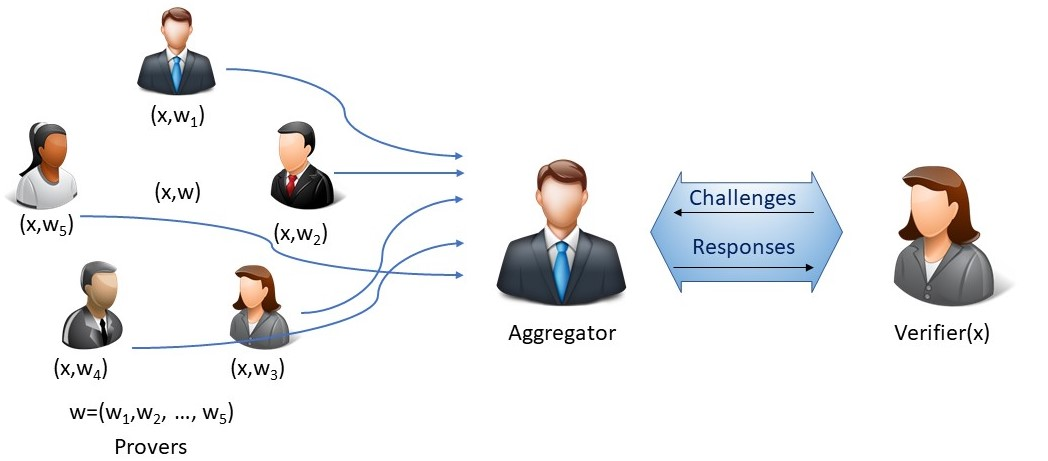
\includegraphics[width=0.9\linewidth]{DPZK.jpg}
%	\caption{Distributed Proof Generation}
%	\label{fig:DPZK}
%\end{figure}

\subsection{Related Notions}
Closely related to our notion is the work of \cite{EfficientTZ} which discusses threshold proofs. This work distributes the prover's side of interactive proofs of knowledge over multiple parties for: (i) improving the security against theft of the user's identity, (ii) improving robustness by ensuring that only a restricted size subset of the provers may be corrupted. The work of \cite{EfficientTZ} primarily captures sigma protocols without allowing interaction among the provers. Our definition captures a broader class of protocols via allowing interaction amongst the provers.  In other words, threshold proofs are a sub-class of the protocols we cater to. Also, other than increasing security via a decentralisation of the prover (or distributing prover's task), our goal is to capture scenarios where multiple provers would like to jointly prove a statement.  Our real-ideal world based definition is inline with MPC style definitions and is more powerful. Pedersen's PhD thesis \cite{Ped92} also defines distributed proofs. Our definition improves the notion of zero-knowledge in \cite{Ped92} where the security model is inherently restricted to a semi-honest collusion of the provers with the verifier. Also, \cite{Ped92} considers the provers' witnesses to always be secret shares of a ``global'' witness and hence the provers' witnesses are \textit{random} when the distributed proof generation begins. But, our definition allows for any distribution on the provers' witnesses, and this impacts some of our security proofs.


%We would like to finally point out that at many scenarios  
%In contrast to the definition in section ~\ref{sec:security model}, all the parties except for the verifier, in the execution of the protocol they may deviate arbitrarily, but the verifier is not allowed to deviate from the protocol. The reason behind considering a preposterously looking adversarial model is that we want to design a zkSNARK which is efficient, secure, publicly verifiable and distributed proof generation property. We know from \cite{}, any interactive honest (public coin) verifier can be transformed into Non-interactive zero-knowledge using \textit{Fiat–Shamir heuristic}. Here the verifier can be semi-honest, i.e., verifier will follow the protocol steps and sends all the challenges uniformly at random.
%-Start with corruption model and give a brief reasoning.
%.\pnote{Describe honest verifier}

\begin{comment}
If all the parties in $\Partyset$ are honest, then the protocol should return 1, this property is called \textbf{\textit{completeness}}.

In this setting, we have two types of corruption models, and that depends on which parties are corrupt:

-- Consider $I$, the set of all corrupt parties consists of all the provers in $\Partyset$, i.e., together they do not have a correct witness for $\stmt$, but they try to cheat in such a way so that the verifier outputs 1. What we want from the protocol is that such a scenario can happen with negligible probability. In other word, whenever in the protocol $\verifier$ outputs 1, then there must be a correct witness $\wit$ such that $\prover_i$ has $\wit_i$ for which $\wit = (\wit_1, \ldots, \wit_{\Num})$, with very high probability. This notion is called \textbf{\textit{proof of knowledge}}. 
	\begin{definition}
		Let $\Func_{\DPZK}$ is the functionality which is defined as ~\ref{func:DPZK} and let $\innp{\Pi}{V}$ is a $\DPZK$ $\Num$-party protocol involving $\Partyset$. We say that $\innp{\Pi}{V}$ realizes $\Func_{\DPZK}$ with computational proof of knowledge property if for every $\ppt$ real world adversary $\Adv$, corrupting at most all provers, there exists a $\ppt$ knowledge extractor $\extrac$ such that for every $\stmt \in L$, for which $\verifier$ outputs 1, $\extrac$ can extract a witness $(\wit_1, \ldots, \wit_{\Num})$ for which $\Func_{\DPZK}$ outputs 1.
	\end{definition}    
	
-- Consider $I$ consists of $\verifier$ and $t$ provers. That is, some of the provers may deviate from the protocol to gain additional information about the honest provers' secret; to achieve this, they may take additional help from $\verifier$'s view. We call a protocol $\innp{\Pi}{\verifier}$ has \textbf{\textit{zero knowledge under t-collusion}}($t$-ZKUC) property, if in this corruption model, corrupted provers and verifier whatever they can compute, the same thing can be computed from the functionality output of the functionality. 
	\begin{definition}
		Let $\Func_{\DPZK}$ is the functionality which is defined as ~\ref{func:DPZK} and let $\innp{\Pi}{V}$ is a $\DPZK$ $\Num$-party protocol involving $\Partyset$. We say that $\innp{\Pi}{V}$ realizes $\Func_{\DPZK}$ with computational zero knowledge under $t$-collusion property if for every $\ppt$ real world adversary $\Adv$, corrupting $I$, at most $t$ provers and verifier, then there exists a $\ppt$ simulator $\Sim$ such that for every $\stmt$, and $\{\wit_i : i\in [\Num]\}$, it holds that: 
		$$\Big\{\Ideal_{\Func_{\DPZK}, \Sim(\secparam),I}(\wit_1, \ldots, \wit_{\Num}) \Big\} \stackrel{c}{\approx} \Big\{ \Real_{\innp{\Pi}{\verifier}, \Adv(\secparam, \wit_T),I}(\wit_1, \ldots, \wit_{\Num}) \Big\}. $$
		Where $\wit_T$ is the input of the corrupt parties.
	\end{definition}

Note that if $I$ consists of the only verifier, then the view of the verifier should not reveal any information about neither the witness nor the inputs of the provers. This notion is called \textbf{\textit{zero knowledge}}, which is subsumed by the notion $t$-ZKUC.
\end{comment}
